\documentclass[11pt, preprint]{aastex}
%%%%%%begin preamble
\usepackage[hmargin=1in, vmargin=1in]{geometry} % Margins
\usepackage{hyperref}
\usepackage{url}
\usepackage{natbib}
\usepackage{graphicx}
\usepackage{amsmath}
\usepackage{amsfonts}
\usepackage{amssymb}
\usepackage{pdfpages} % breaks with aastex6
\usepackage{import}
\usepackage{wrapfig}

\usepackage{color}
\hypersetup{
  colorlinks   = true,
  %citecolor    = blue
  citecolor    = gray
  % gray is not being found!?!
  % gray is found if pdfpages is used... crap.
  %citecolor    = grey
  %citecolor    = Gray
}

\setcounter{tocdepth}{2}
%% headers
\usepackage{fancyhdr}
\pagestyle{fancy}
\lhead{}
\renewcommand{\headrulewidth}{0pt}
%\pagenumbering{gobble}
%\renewcommand*{\thefootnote}{\fnsymbol{footnote}}

\renewcommand{\vec}{\ensuremath{\boldsymbol}}
\newcommand{\dedalus}{\href{http://dedalus-project.org}{Dedalus}}
\newcommand{\del}{\ensuremath{\vec{\nabla}}}
\newcommand{\scrS}{\ensuremath{\mathcal{S}}}

\newcommand{\nosection}[1]{%
  \refstepcounter{section}%
  \addcontentsline{toc}{section}{\protect\numberline{\thesection}#1}%
  \markright{#1}}
\newcommand{\nosubsection}[1]{%
  \refstepcounter{subsection}%
  \addcontentsline{toc}{subsection}{\protect\numberline{\thesubsection}#1}%
  \markright{#1}}

\usepackage{atbegshi}
%%%%%%end preamble


\begin{document}
\title{Convective Conundrums in the Asteroseismic Age:\\The interplay of rotation and magnetism in stellar convection}
\vspace{-0.5cm}
\maketitle
\thispagestyle{fancy}

\vspace{-0.8cm}
\begin{flushleft}
  \textit{Principal Investigator:} Evan H. Anders 
\end{flushleft}

\vspace{-1.3cm}

\section{Motivation}
\sectionmark{Motivation}
\vspace{-11pt}

\paragraph{Asteroseismology}
\label{sct:asteroseismology}
The advent of asteroseismic science has closely paralleled that of exoplanetary science.
Early ground-based observations of stellar pulsations \citep[e.g.,][]{kjeldsen&frandsen1991, bouchy&carrier2001, bedding&all2001} have given way to datasets larger than $10^4$ stars \citep[e.g.,][]{yu&all2018, santos&all2019b} in the age of CoRoT, Kepler, and K2 data.
Another 20,000 asteroseismically-interesting targets are being observed in the TESS satellite's two-year mission \citep{schofield&all2019}.
By 2030 we expect to have observed $10^7$ pulsating red giants and $10^5$ dwarfs and subgiants \citep{huber&all2019}.
In addition to teaching us about the nature of stellar interiors, asteroseismology enables the accurate measurement of stellar ages, masses, and radii, which in turn facilitates studies in galactic archaeology and exoplanetary measurements.
Asteroseismic measurements generally rely on one-dimensional (1D) stellar structure models, and these models have some known deficiencies \citep{buldgen2019}, in particular their handling of three-dimensional (3D) dynamical phenomena like convection, rotation, and magnetism.
The exponential rise in asteroseismic targets demands a continued investment in the theory that informs these stellar models and asteroseismic measurements.

State-of-the-art stellar strucuture models are produced by 1D codes like MESA \citep{paxton&all2011}.
Unfortunately, MESA models necessarily depend on 1D parameterizations of convection and often employ the decades-old mixing length theory \citep[MLT,][]{bohm-vitense1958}.
While some aspects of convection are adequately described by MLT, it fails in a number of situations.
For example, 1D stellar models incorrectly produce pulsations in the surface layers of Sun-like stars, while 3D models of convection in these layers fare better \citep{jorgensen&weiss2019}.
Additionally, 1D models assume spherical symmetry and generally neglect magnetic and rotational effects.
Observations of stellar flares \citep{kowalski2016} and magnetically-induced pulsational frequency shifts \citep{santos&all2018} suggest that magnetism should not be neglected.
Furthermore, the Sun exhibits differential rotation characterized by latitudinal variations in angular velocity within the solar convection zone \citep{thompson&all1996, schou&all1998}, and latitudinal differential rotation has now been observed in other stars \citep{benomar&all2018}.
Together, these observations suggest that 1D parameterizations of convection which neglect complicating effects cannot sufficiently capture the complexities of stars.
In order to properly and fully utilize abundant asteroseismic data, we must improve the models on which asteroseismic inversions rely.

\vspace{-0.5cm}
\paragraph{The Solar Convective Conundrum}
\label{sct:convective_conundrum}
The outer 30\% of the Sun is a highly stratified convective envelope, and recent observations reveal that we lack a fundamental understanding of dynamics in this region.
Various helioseismic observations \citep{hanasoge&all2012, greer&all2015} detect convective velocity magnitudes which vary by two orders of magnitude.
Furthermore, these observations, as well as measurements of solar surface velocities \citep{hathaway&all2015}, have an unexpected absence of velocity at large spatial scales.
In short, we do not observe large-scale ``giant cells'' driven by buoyant motions deep in the solar convection zone.
These measurements, and the absence of giant cells, consitute the Solar Convective Conundrum.

Two primary hypotheses currently aim to explain the absence of giant cells: ``entropy rain'' and a rotationally constrained solar convective interior.
The entropy rain hypothesis, first suggested by \citet{spruit1997}, posits many theories over-predict the importance of upflows and that \emph{downflows} are predominantly responsible for carrying the solar luminosity across the solar convection zone.
Recent theory and simulations, including some of my own work, suggest that small, intense downflows can indeed traverse the entire convection zone intact and may be more important than upflows in solar-like convection \citep{brandenburg2016, kapyla&all2017, andersLB2019}.
To date, this work neglects magnetism and rotation, and it is unclear how these complicating effects interact with these fast, powerful downflows.
Meanwhile, the rotationally constrained interior hypothesis suggests that Coriolis forces dominate the dynamics of deep solar convection, and that these forces mask giant cells.
Simulations by \citet{featherstone&hindman2016} show that as convective flows become more rotationally constrained, dominant convective velocities are pushed to smaller length scales.
However, rotational effects on simulations can be hard to quantify; some simulations which nominally rotate at the solar rate show \emph{anti-solar} differential rotation \citep{gastine&all2014}, and other rotationally constrained simulations exhibit Jupiter-like bands \citep{brun&all2017}.
Regardless, current results and hypotheses suggest that the interplay between downflows and rotational effects must be better understood in stellar convection.

\vspace{-0.5cm}
\paragraph{Modern convective simulations}
\label{sct:modern_simulations}
The earliest simulations in stellar-like convection \citep{graham1975, hurlburt&all1984, cattaneo&all1991, brummell&all1996, brummell&all1998} often sought to study simplified systems.
Cartesian geometry was employed, and convective flows in the presence of one or more complicating effects (stratification, rotation, magnetism, etc.)~were explored.
Despite vast modern computational resources, similar studies \citep[e.g.,][]{wood&brummell2012, anders&brown2017, wood&brummell2018} have become rare in the past two decades, and the highly laminar results of simulations from twenty years ago are often the state-of-the-art.

Recently, numericists have often switched aims from simply understanding convection to trying to reproduce precisely aspects of solar or stellar convection.
Small scale ``local'' simulations with realistic radiative transfer strikingly visually resemble solar surface convection and sunspots \citep{stein&nordlund1998, rempel&all2009, stein&nordlund2012, rempel2014}.
Local simulations have shaped how some observational experts interact with simulations, and the raw data of \citet{rempel2014}'s simulations are being used directly as high-resolution observations of solar convection \citep[see e.g.,][and others]{vankooten&cranmer2017, shchukina&trujillo2019}.
While simulations of solar surface convection reproduce solar features remarkably well, simulations of deep convection fail to reproduce observations  \citep{hanasoge&all2015}.
These global simulations exhibit giant cells as well as cycling dynamos and latitudinal differential rotation with very different timescales and profiles than those of the Sun \citep{brown&all2010, brown&all2011, guerrero&all2016, hotta&all2016, brun&all2017, strugarek&all2018}.
Simple simulations, where effects like rotation and magnetism can be well understood, should be utilized to understand why deep global simulations fail to reproduce solar observations.
This understanding can in turn be used to produce better ``realistic'' simulations which more accurately reflect aspects of true solar convection.
Realistic simulations built on a more detailed fundamental understanding of stellar convection can produce valuable synthetic observables for helioseismologists, asteroseismologists, and scientists who will soon use the NSF's Daniel K. Inouye Solar Telescope (DKIST) to study the solar surface at high resolution.


\section{Intellectual Merit}
\vspace{-11pt}
\sectionmark{Intellectual Merit}

\label{sct:intellectual_merit}

\paragraph{Rotating magnetoconvection across all scales}
Over the course of my postdoctoral studies, I will take advantage of the flexibility of the Dedalus pseudospectral framework \citep{burns&all2019}, which I have used throughout my graduate career, to study numerical simulations at three different scales.
In task A, I will study simulations of discrete events, or thermals \citep[as in][]{andersLB2019}, which model individual stellar convective downflows and can achieve high levels of turbulence.
In task B, I will study simulations of mesoscale convection \citep[as in][]{anders&brown2017} to gain an understanding of how these effects behave in the presence of the convective-radiative interface at the base of a solar-like convective zone.
In task C, I will study simulations of global stellar convection \citep[as in][]{lecoanet&all2019}, developing and using new community tools to study the importance of rotation and magnetism over Kelvin-Helmholtz timescales.
Each task is expected to take one full year of my three-year postdoctoral fellowship.

\vspace{-0.8cm}
\subsection*{Task A: Dynamics of individual downflows}
\vspace{-0.3cm}
\label{sct:taskA}
\begin{wrapfigure}{l}{0.35\textwidth}
	\begin{center}
	\vspace{-30pt}
    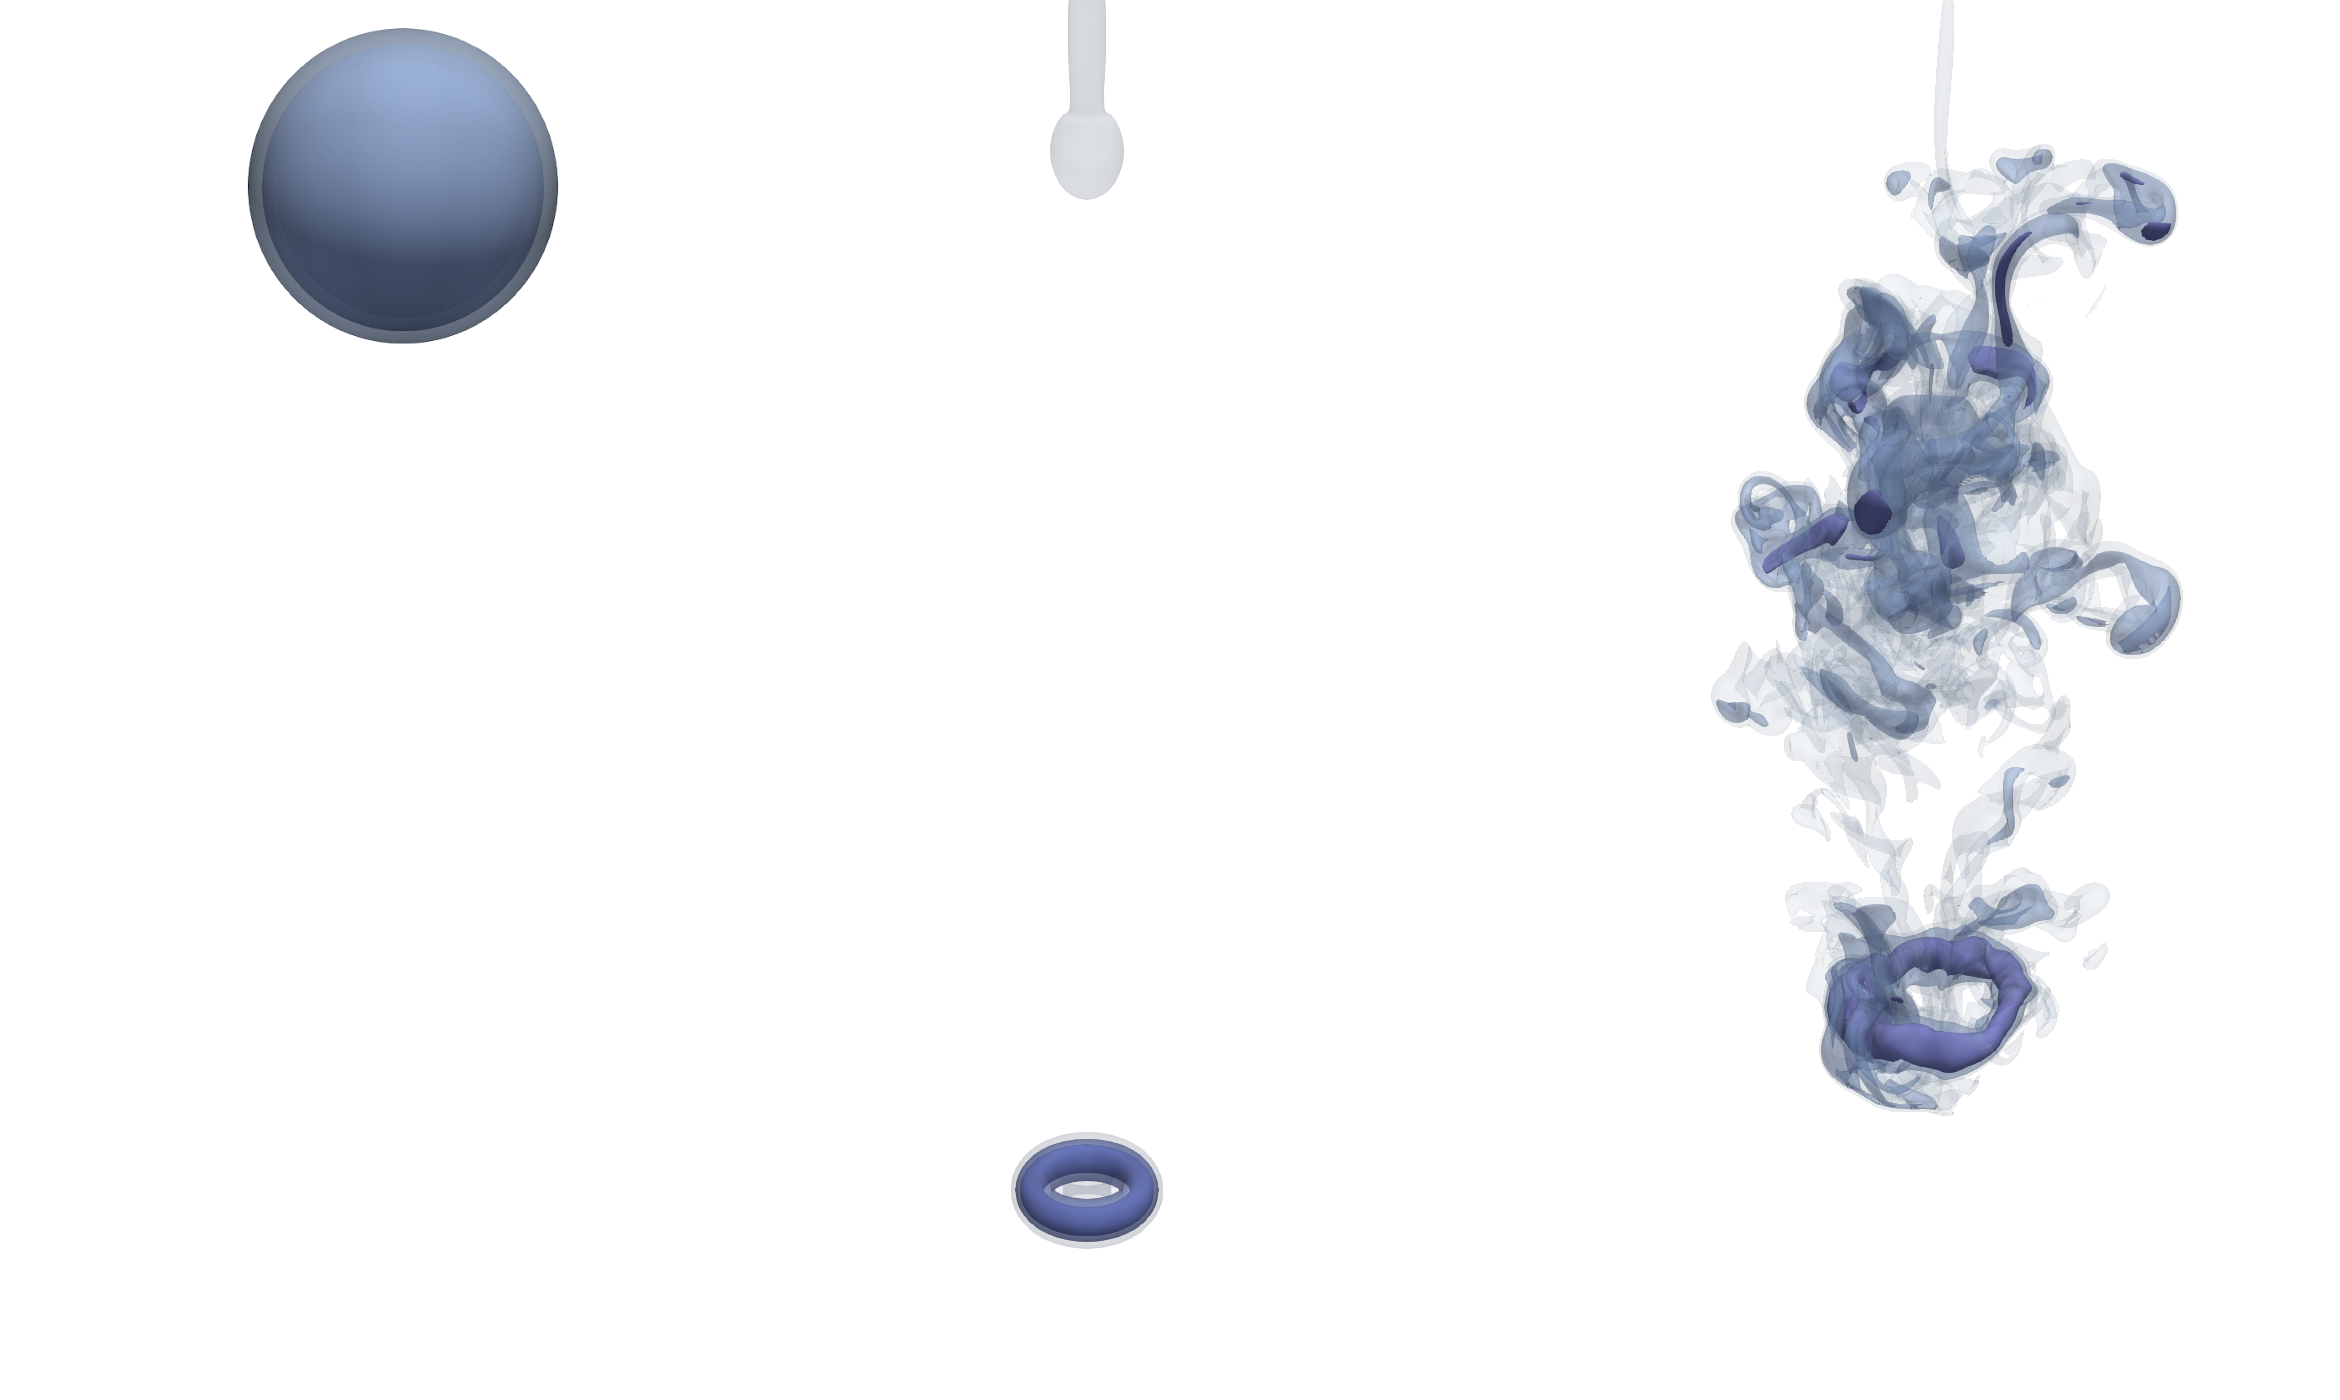
\includegraphics[width=0.34\textwidth]{./figs/thermals_comparison.png}
	\vspace{-20pt}
	\end{center}
    \caption{
	3D visualizations of entropy perturbations in the downward-propagating reference frame of evolved laminar (left) and turbulent (right) thermals.
	\label{fig:thermals_comparison} }
	\vspace{-11pt}
\end{wrapfigure}

In the envelopes of lower main sequence stars, convection occurs in the presence of extreme stratification.
Stratified convection is characterized by powerful, localized downflows, and broad, slow upflows.
Recent theory and observations \citep[e.g.,][]{hanasoge&all2015, brandenburg2016, kapyla&all2017, andersLB2019} suggest that downflows may be the predominant mechanism for transporting stellar luminosity in these convective zones.
Furthermore, \citet{tobias&all1998} showed that downflows can effectively pump magnetic fields downwards in certain regimes.
These results suggest that downflows in stratified convection deserve careful study.

Downflows may turbulently break up into distinct pieces as they fall and these pieces can be modeled as thermals.
Thermals are regions of cold fluid which accelerate due to buoyancy forces and shape themselves into vortex rings; evolved thermals are visualized in Fig. \ref{fig:thermals_comparison}.
Thermals are observed and studied in the Earth's atmosphere and are well understood in the Boussinesq limit.
%Recently, I studied thermals as a model for solar convection and came to understand the effects of stratification on the propagation of thermals \citep{andersLB2019}.

Thermals provide a useful model of stellar downflows because they can be modeled analytically and simulated.
Hydrodynamic thermals in stratified domains are fully specified by: (a) the stratification of the background atmosphere and (b) whether they are laminar or turbulent.
My work in \citet{andersLB2019} determined the influence of stratification on thermals, and in the Boussinesq regime, \citet{lecoanet&jeevanjee2019} showed that turbulence does not appreciably change the evolution of thermals.
I now propose to study thermals in a fixed high-stratification regime to learn how magnetism and rotation affect their evolution.
Over the course of Task A, I will try to answer two fundamental questions about stellar downflows:
\vspace{-16pt}
\begin{enumerate}
\item Can stellar downflows transit the full depth of their convective envelopes, or do rotational or magnetic processes inhibit their propagation?
\vspace{-10pt}
\item How much energy do downflows transport, and in which regimes do rotational and magnetic effects change their energy fluxes?
\end{enumerate}

\paragraph{Task A.1: Rotational filtering of downflows}
\label{sct:taskA1}
I will study the effects of rotation on thermals in simple Cartesian \emph{f-plane} domains.
These plane-parallel atmospheres model a fixed latitude where flows experience Coriolis forces from global rotation.
I will study downflows at the equator, poles, and mid-latitudes.
At each of these latitudes, I will study flows which experience varying degrees of rotational constraint.
I will study many laminar thermals to broadly characterize rotational effects before simulating select turbulent simulations in regimes which exhibit distinctly different behavior.
The primary goal of these studies will be to determine at various latitudes how strong rotation must be to prevent thermals from transiting the convection zone and therefore transporting the solar luminosity.

\vspace{-0.7cm}
\paragraph{Task A.2: Magnetic filtering of downflows}
\label{sct:taskA2}
I will study thermals in the presence of magnetism but absence of rotation.
The inclusion of magnetism requires a choice of initial magnetic field geometry, and I will study both cases in which there is a uniform background field and where there is a thin horizontal sheet of magnetism for the thermal to pass through \citep[as in][]{tobias&all1998}.
I will vary the orientation and strength of the initial magnetic fields in a manner analagous to the rotational simulations in Task A.1.
This work will be the magnetic complement to Task A.1, further constraining regimes in which downflows can effectively propagate through a stellar convection zone to transport the stellar luminosity.


\vspace{-0.8cm}
\subsection*{Task B: Mesoscale interactions at the radiative-convective boundary}
\vspace{-0.3cm}
\label{sct:taskB}
In solar-like stars, the strongly stratified convective zone overlies a stable interior radiative zone.
In the Sun, the radiative-convective boundary (RCB) is characterized by a transition from moderate instability to strong stability.
Now that downflows are considered a key element of stellar convection, it is crucial to understand how these downflows interact with the RCB.

Helioseismic measurements suggest that the RCB is very thin, occupying only $\sim$5\% of a pressure scale height at the base of the convection zone, or $\sim$1\% of a solar radius \citep{basu1997}.
Simulations often produce RCBs which are too thick or too thin by up to an order of magnitude \citep[see e.g.,][]{hotta2017, kapyla2018}.
This suggests that these simulations are in the wrong stiffness regime \citep{brummell&all2002, couston&all2017}, or that convective motions run into too hard or soft of an interface.
The effects of magnetism can furthermore appreciably alter deep velocity magnitudes which in turn alter RCB widths \citep{hotta&all2015}.
It is widely thought that dynamics in the RCB are a critical ingredient in generating the Sun's magnetic dynamo, and so understanding the effects of a too-thick or too-thin RCB is crucial.
The goal of this task is to determine how angular momentum and magnetism are pumped into the RCB as a function of RCB stiffness.



\vspace{-0.5cm}
\paragraph{Task B.1: The critical magnetic field strength}
\label{sct:taskB1}
\begin{figure*}[t!]
    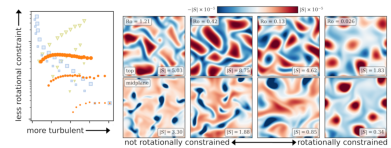
\includegraphics[width=\textwidth]{./figs/rossby_plot.png}
	\vspace{-1cm}
    \caption{(left, Fig 1b of \citet{anders&all2019}) The degree of rotational constraint is difficult to predict as a function of turbulence in convective simulations.
	Rotational influence changes as turbulence is increased along traditional paths through parameter space (green triangles and blue squares).
	We discovered a new parameter which, when held constant (orange circles) fixes the rotational influence.
	(right eight panels, Fig. 2 of \citet{anders&all2019}) Increasing rotational constraint (from left to right) changes traditional convective patterns to vortical columns with little difference between the top and midplane of the atmosphere (top vs. bottom row).
	It is crucial to simulate solar convection under the same rotational influence as the real Sun to ensure that flow topologies and interactions accurately model solar flows.
	\label{fig:rossby_plot} }
	\vspace{-0.3cm}
\end{figure*}

Convective flows in the presence of a strong magnetic field will be appreciably affected by that field.
Similarly, a weak magnetic field will not noticeably affect convective motions.
A ``critical'' field strength at which convection passes from weakly to strongly affected by magnetism separates these regimes.
Observationally, one would expect stars with more vigorous convection to have a higher critical field strength, and hotter stars will likely have more vigorous convection and higher critical field strengths.
Unfortunately, the mapping of this intuition to simulations is not straightforward, and it is difficult to predict simulation flow regimes \emph{a priori}.
The goal of this subtask is to determine the critical field strength.

An analagous argument can be made for rotating convection, where rapid global roation modifies convective flows and slow rotation does not.
During my PhD studies, I identified the critical angular frequency in convective simulations \citep[][and Fig. \ref{fig:rossby_plot}]{anders&all2019}.
Convective flow fields look vastly different when you are far below, close to, or far above the critical angular frequency, and the same is likely true for the critical magnetic field.
I will employ similar methods to those in \citet{anders&all2019} to complete this subtask, and this knowledge will help numericists more precisely study solar-like flows with the proper force balances.

\vspace{-0.7cm}
\paragraph{Task B.2: Downflow interactions at the RCB}
\label{sct:taskB2}
In this task, I will study how downflows pump angular momentum and magnetism into or across the RCB.
I will study very stiff RCBs, which act similar to hard walls, and very soft RCBs which convective motions can easily pass through.
Using the knowledge gained in tasks A and B.1, I will only study simulations in the magnetic and rotational regimes where downflows can transit the full convection zone.
\citet{tobias&all1998} showed that convective downflows can effectively pump magnetic fields across soft RCBs.
Here I will extend that work to include turbulent flows and stiff RCBs to determine the regimes in which magnetic fields and angular momentum can be pumped into the RCB.
The observations of a thin RCB \citep{basu1997} suggest that the solar RCB is quite stiff, but it is widely believed that shearing motions in the solar RCB are a critical piece of the solar dynamo.
If downflows cannot pump magnetic fields into a stiff RCB, then a different mechanism may be responsible for generating new magnetic fields.
I will also investigate if a stiff RCB could potentially insulate the solar radiative interior from convectively-driven angular momentum transport, which could help explain why the solar differential rotation profile gives way to a uniformly rotating interior beneath the RCB.

\newpage
\subsection*{Task C: Global studies in relaxed atmospheres}
\vspace{-0.3cm}
\label{sct:taskC}

\begin{wrapfigure}{r}{0.3\textwidth}
	\begin{center}
	\vspace{-14pt}
    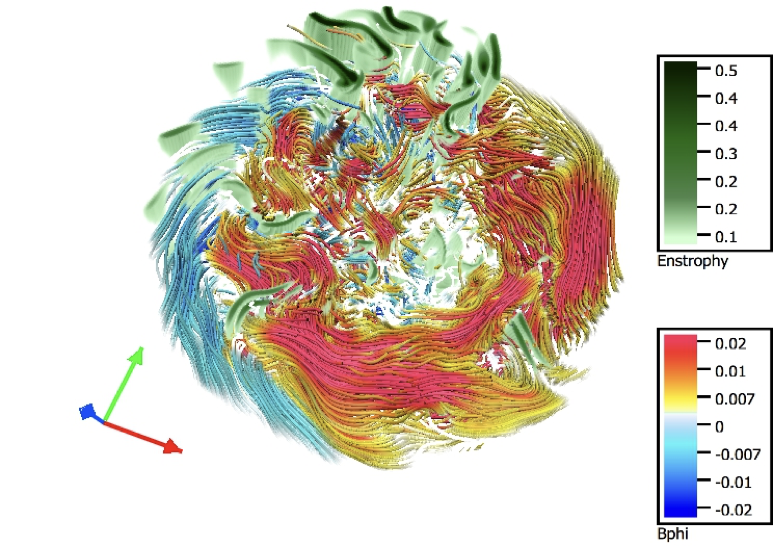
\includegraphics[width=0.28\textwidth]{./figs/mdwarf.png}
	\vspace{-16pt}
	\end{center}
    \caption{A volume rendering of a Dedalus global dynamo simulation.
	Green surfaces show enstrophy, or the squared vorticity.
	Red and blue lines show the azimuthal magnetic field magnitude.
	\label{fig:mdwarf} }
	\vspace{-6pt}
\end{wrapfigure}
The advances made in Tasks A \& B will culminate in examining convection at the largest scales in global spherical simulations of rotating magnetoconvection.
Dedalus is capable of accurately simulating global domains which include the origin at $r = 0$ \citep{lecoanet&all2019}; a visualization of basic outputs from these simulations is shown in Fig. \ref{fig:mdwarf}.
One major barrier to performing turbulent global simulations is that they are costly.
Some of these costs are unavoidable because highly resolved, turbulent simulations necessarily take small timesteps, and therefore simulation times are very long.
However, some of the expense of these simulations is time wasted waiting for simulation equilibration or relaxation.
For example, the thermal structure of the Sun evolves over a Kelvin-Helmholtz timescale of $10^7$ years, which is significantly longer than the five minute convective overturn time of solar surface convection \citep{anders&all2018}.
As simulations approach the turbulent regime of stars, relaxation and dynamical timescales separate and traditional methods force numericists to choose between state-of-the-art turbulence \emph{or} equilibrated dynamics---but not both.

The goal of task C is to enable studies of equilibrated global dynamo simulations which exhibit state-of-the-art turbulence.
To accomplish this, I will develop and test a community tool which accurately takes timesteps on the order of relaxational timescales.
During my graduate career, I developed and studied such a tool in a very simple convective systems \citep{anders&all2018}, and here I will extend it to global dynamo simulations.
This work showed that a tool like the one I am proposing here can be feasibly implemented and tested for accuracy.
Furthermore, this tool used an order of magnitude less computer time than standard timestepping on a turbulent simulation by skipping this equilibration timescale.

\vspace{-0.5cm}
\paragraph{Task C.1: Accelerated evolution of global simulations}
\label{sct:taskC1}
The goal of this subtask is to extend my accelerated evolution method to rapidly equilibrate thermodynamic and angular momentum profiles in global simulations.
The foundational work of task A will help determine which equation forcings will be important in different regimes and the work of task B will help determine how to set up this tool near RCB-like interfaces.
As in \citet{anders&all2018}, I will compare this tool's outputs to simulations which run for equilibration timescales to build trust in the method.
This module will be made public, and will be flexibly designed so that users of codes beyond Dedalus can benefit from its computational speed-ups.

This accelerated evolution tool could have great benefits for asteroseismic research.
Recently, \citet{jorgensen&weiss2019} coupled previously computed global simulations with 1D stellar structure tools to circumvent some of MLT's problems.
This 3D-to-1D coupling cannot currently be done for arbitrary stars due to the expense of global simulations. 
The tool proposed here will be able to relax global simulations of arbitrary stars to further enable these 3D-to-1D efforts and improve the stellar structure models available to observers.


\paragraph{Task C.2: Relaxed simulations of the solar dynamo}
\label{sct:taskC2}
I will study global simulations of the solar convection zone in regimes where flows feel solar-like effects of both rotation and magnetism, using the knowledge from task B.1 to determine how to set up such simulations.
Using the tool developed in task C.1, I will accelerate the evolution of these simulations.
The goal of these simulations will be to examine the relaxed differential rotation profiles that appear in different rotational regimes, and how these differential rotation profiles affect the time evolution of the magnetic dynamo.
Many modern dynamo simulations measure the evolution of magnetic fields during the equilibration process due to computational limitations.
It is likely that the time-dependent dynamo behavior of simulations is strongly influenced by the underlying evolution of the mean state, and these simulations will examine dynamos without any mean state drift.


\vspace{-0.8cm}
\subsection*{Computational Feasibility}
\vspace{-0.3cm}
\label{sct:feasibility}
Tasks A-C are arranged from least to most computationally expensive.
Based on my work in \citet{anders&brown2017, anders&all2018, anders&all2019}, Dedalus takes $\mathcal{O}(10^3)$ cpu-sec per iteration for a run with a grid resolution of 384$^3$ on a system comparable to NASA Pleiades.
Task A simulations will each take $\mathcal{O}(10^4)$ iterations, while turbulent runs in tasks B and C will take $\mathcal{O}(10^6)$ iterations each.
Laminar and turbulent simulations of thermals thus cost roughly 5000 and $10^5$ cpu-hours each, respectively.
State-of-the-art simulations in tasks B and C will cost roughly $10^6$ cpu-hours each.
The projects described here total 5-10 million cpu-hours per year in tasks B and C, with less (2-3 million cpu-hours) in the first year while thermals are being studied.
I will be able to run the simulations in task A on Northwestern's 11,800-core Quest supercomputer.
I will leverage my AAPF fellowship and apply for time on NSF XSEDE resources such as Stampede2, Comet, or Bridges to to allow for larger scale runs in tasks B and C. 

\vspace{-0.8cm}
\subsection*{Collaborative studies at CIERA}
\vspace{-0.3cm}
\sectionmark{CIERA}
\label{sct:ciera}
Northwestern university, and specifically the Center for Interdisciplinary Exploration and Research in Astrophysics (CIERA), is the perfect location for me to carry out this proposed work.
Prof.~Daniel Lecoanet, who will be my primary advisor and collaborator, is a core developer of Dedalus.
His expertise using Dedalus and his past work on thermals \citep{lecoanet&jeevanjee2019, tarshis&all2018}, convection \citep{lecoanet&quataert2013, lecoanet&all2014, couston&all2017}, rotating convection \citep{couston&all2019}, and global simulations \citep{lecoanet&all2019} will make him a valuable collaborator and advisor for the projects proposed here.
Furthermore, I have already published a paper on thermals in close collaboration with Prof.~Lecoanet \citep{andersLB2019}, so task A will serve as an excellent transition project into my postdoctoral studies on my arrival.
In addition to Prof.~Lecoanet, Prof.~Yoram Lithwick would be an excellent partner for collaboration due to his work on rotating convection \citep[e.g.,][]{BDLithwick2014}.
CIERA houses many experts in computational fluid dynamics beyond Profs.~Lecoanet \& Lithwick, such as Profs.~Sasha Tchekhovskoy \& Claude-Andre Faucher-Giguere.
I look forward to joining the astrophysical fluid dynamics group at CIERA where I will have many opportunities to discuss and develop new numerical techniques, strategies, and applications across astrophysics.


Furthermore, in addition to the focused educational and outreach projects described below in section \ref{sct:broader_impacts}, CIERA will provide me with numerous small scale opportunities to participate in public outreach.
CIERA's Astronomy on Tap program as well as its CIERA Astronomer Evenings provide bite-sized and accessible ways to interact with public audiences.
Dearborn Observatory's observation tours are very similar to the public open houses I helped host at CU Boulder's Sommers-Bausch observatory.
The state-of-the-art Adler planetarium also provides similar opportunities such as its `Scopes in the City program or its Space Visualization Lab astronomy conversations.


\vspace{-17pt}
\section{Broader Impacts}
\vspace{-11pt}
\sectionmark{Broader Impacts}
\label{sct:broader_impacts}

\paragraph{Motivation}
A majority of high school students across Illinois and in Chicago do not meet science and math standards.
In 2017-2018, only roughly 40\% of high schoolers received a score deemed proficient on the Illinois Science Assessment and fewer were considered proficient on their math SAT scores \citep{irc2018}.
Numerous outreach programs which involve short-lived visits to high schools aim to address these problems and seem to positively improve STEM attitudes and engagement at the high school level \citep{vennix&all2017, vennix&all2018}.
Feedback from high school educators regarding these programs identified the expertise of the visiting scientists on the topics they teach as one of the reasons these programs can be successful \citep{laursen&all2007}.

At the university level, practices in physics education are an active subject of research.
Physics courses rely heavily on lectures, but evidence now shows that lecturing must be combined with alternate modes of instruction to reach desired learning outcomes \citep{meltzer&thornton2012}.
Furthermore, student attitudes regarding science regress towards less favorable responses over the course of traditional introductory lecture courses in science \citep{reddish&all1998}.

Science education clearly faces struggles in achieving desired outcomes at both the secondary and post-secondary levels.
However, improved STEM engagement has been seen in high schools when topical experts are involved in course design, and improved physics learning outcomes have been measured at the university level when modern teaching pedagogical techniques are applied.
During my time at CIERA, I will bring together local experts on teaching pedagogy (high school teachers) and physics (graduate students at CIERA) to share knowledge and collaboratively design course modules leading to improved learning outcomes at the secondary and post-secondary levels.

\vspace{-0.5cm}
\paragraph{Improving physics education outcomes through sharing of expertise}
I will create a workshop series which partners experts in scientific content (graduate students at CIERA) and pedagogy (high school teachers).
The product of this series will be pedagogically- and scientifically- sound teaching modules that can be used in high school classrooms across the Chicago area and the nation.
The participating pedagogy experts will identify content areas that their students struggle to learn and will define the specific learning outcomes of these modules using Next Generation Science Standards (NGSS) disciplinary core ideas in physics.
Small groups consisting of at least one pedagogical and one scientific expert will be formed around each module.
During development, an NGSS scientific practice will be identified and incorporated into each module to provide students with opportunities to participate in scientific practices while learning scientific ideas.

This workshop series will meet once or twice a week for 2-3 hours apiece over the course of ten weeks.
These workshops will take place during the summer quarter, when high school educators and graduate student schedules are most flexible.
Individual workshop meetings will consist of a large-group lesson in teaching pedagogy followed by small-group work on module development in which that pedagogical lesson is applied.
This format will enable graduate student participants to learn pedagogical lessons and then immediately see them applied while they gain an understanding of the intricacies of curriculum design.
To help encourage participation, I will use funds from my fellowship allowance to provide participants with free parking passes, lunches, and coffee/tea.

These workshops will expose young career scientists to some basic teaching pedagogical research which they will be able to employ at the university level in their careers.
Furthermore, these workshops will expand the scientific content knowledge of participating high school teachers in a self-identified area of teaching difficulty.
On a larger scale, this program will produce well-informed teaching modules which can be used widely in high schools, and will leverage connections and input from high school teachers to help ensure adoption of these modules.

\vspace{-0.5cm}
\paragraph{Collaborative development}
\label{sct:development}
I will develop my workshop series in collaboration with Ms. Michelle Paulsen, CIERA's Director of Education, Outreach, and Communications Programs.
Ms.~Paulsen has experience as a high school physics teacher and has been the chair of a large suburban high school's science department.
Furthermore, Ms.~Paulsen has been instrumental in the creation of CIERA's RCTP program, which helps young career scientists develop presentation skills over the course of a ten-week workshop series similar to the one I propose here.

Participation from educators will be crucial for the success of the program proposed here.
I will partner with local teacher organizations such as Physics Northwest, the Illinois State Physics Project (ISPP), and the Chicago Section of the American Association of Physics Teachers (CSAAPT).
Physics Northwest's monthly meetings, ISPP's quarterly meetings, and CSAAPT's biannual meetings will be excellent venues in which to advertise the program and build a professional network of interested educators in the Chicago area.
Furthermore, CIERA's Reach for the Stars program, an NSF GK-12 program, has partnered with many local area high schools over the past decade and will serve as an excellent in-house link to this audience.

The capstone of this workshop series for high school educators will be the production and use of these modules in their own classrooms.
However, graduate students participants do not have their own high school classroom to return to.
Fortunately, CIERA has a close connection with the Chicago Public Library system, where CIERA graduate students run data science clubs for interested area high school students.
I will partner with the library, CIERA, and these clubs to create a venue where graduate student participants of my workshop series can teach their module.

\vspace{-0.5cm}
\paragraph{Module distribution \& workshop outcomes} 
I will work to ensure distribution of the produced modules beyond the classrooms of my participating pedagogical experts.
In my later years at CIERA, I will advertise the created modules at the meetings of Physics Northwest, ISPP, and CSAAPT.
Modules will furthermore be made publically available on the American Association of Physics Teachers online ComPADRE system, which stores resources for physics and astronomy educators and is publically available.
These modules will also be made available on CIERA's website, similar to products from current programs like Reach for the Stars are.
 \vspace{2pt}\\
In summary, this workshop series will: 
\vspace{-14pt}
\begin{enumerate}
\item Expose interested graduate students at CIERA to best practices in teaching pedagogy, and provide those students with a teaching experience.
\vspace{-9pt}
\item Expand content knowledge of high school educators while providing them with a strong lesson plan to employ on a topic that their students struggle to learn.
\item Connect university scientists with teachers and teaching organizations in the greater Chicago area to create lasting partnerships between scientific and pedagogical experts.
\vspace{-9pt}
\item Distribute widely applicable teaching modules appropriate to the high school level which simultaneously teach core ideas and scientific practices, as defined by NGSS.
\vspace{-9pt}
\end{enumerate}



\vspace{-22pt}
\section{Personal career growth and development}
\vspace{-11pt}
\label{sct:personal_growth}
My graduate education has given me numerous opportunities to develop as a researcher, a teacher, and a member of my workplace community; see my biographical sketch for a brief description of some of these experiences.
I know from these experiences that I enjoy teaching and research equally, which has affirmed my career goal to become a professor at the university level.
My proposed activities build naturally on research, outreach, teaching, and professional development work that I carried out as a graduate student, and will be feasibly accomplished over the next three years.
I am excited about the opportunity to work with Prof.~Lecoanet, and I look forward to the new theoretical knowledge, computational tools, and pedagogical tools I will gain while growing as a researcher and teacher at CIERA.

\vspace{-33pt}
\section{Timeline}
\vspace{-11pt}
Task A will occupy my research time during my first year; during this time I will also establish (fall through spring quarter) and teach (summer quarter) the first iteration of my yearly teaching workshop series.
Task B will occupy my time during my second year, during which time I will iterate upon my workshop series and advertise the products of the first series. 
In my third year at CIERA, I will complete task C while I work to ensure that my workshop program transitions to new leadership when I leave so that future students can continue to reap its benefits.

\vspace{-30pt}
\section{Summary and Perspectives}
\vspace{-11pt}
Observations of pulsating stars are plentiful but require 1D models which depend upon simple parameterizations of convection.
Unfortunately, observations of the Sun have revealed that our parameterizations and fundamental understanding of stellar convection are flawed.
Numerical simulations have been useful tools for establishing our understanding of stellar convection and modeling observations, but modern simulations poorly reproduce deep flows in the Sun.
Simplified simulations should be employed to explain these troubling observations.

The simulations proposed here are necessary and timely.
Current convective models cannot explain the Convective Conundrum and the combined effects of downflows, rotation, and magnetism is unclear and has not been well explored.
An understanding of these effects can help improve the underlying stellar structure models used in the ever-growing field of asteroseismology.
Furthermore, these studies will ensure that convective simulations accurately model flows in the stellar regime, which is crucial at a time when simulations are increasingly being treated as obervations.
The fundamental problems presented here are of broad scientific interest, but are specifically topics of NSF investigation, as evidenced by the NSF's support for the DKIST telescope which will soon come online.
The collaborative studies centered at CIERA will address the following key questions:
\begin{itemize}
\vspace{-12pt}
\item How strong do rotation and magnetism have to be to prevent entropy rain---and stellar downflows---from being a dominant dynamical process?
\vspace{-7pt}
\item Is the interaction of downflows with the radiative-convective boundary responsible for stellar differential rotation and stellar magnetic dynamos?
\vspace{-7pt}
\item How do we avoid wasting computational resources on equilibration, and how does equilibration affect large-scale convective dynamo properties?
\end{itemize}



\newpage
\AtBeginShipout{%
\AtBeginShipoutDiscard
}
\setcounter{page}{1}
\nosection{References}
\bibliographystyle{apj_title}


%\newpage
%\bibliographystyle{apj_title}
\bibliography{biblio}
\end{document}
